\documentclass[journal]{IEEEtran}
\IEEEoverridecommandlockouts
% The preceding line is only needed to identify funding in the first footnote. If that is unneeded, please comment it out.
\usepackage{cite}
\usepackage{amsmath,amssymb,amsfonts}
\usepackage{algorithmic}
\usepackage{graphicx}
\usepackage{textcomp}
\usepackage{xcolor}
\def\BibTeX{{\rm B\kern-.05em{\sc i\kern-.025em b}\kern-.08em
    T\kern-.1667em\lower.7ex\hbox{E}\kern-.125emX}}
\begin{document}

\title{Predicting University Rankings on the US Faculty Hiring Networks via GNNs
\thanks{Final project report for the \textit{Network Machine Learning} course}
}

\author{\IEEEauthorblockN{\textbf{Junwu Chen}} \\
\IEEEauthorblockA{\textit{Laboratory of Artificial Chemical Intelligence (LIAC)} \\
\textit{Institute of Chemical Sciences and Engineering }\\
\textit{Ecole Polytechnique F\'{e}d\'{e}rale de Lausanne (EPFL)} \\
Lausanne, Switzerland \\
junwu.chen@epfl.ch}
}

\markboth{Final project report for the \textit{Network Machine Learning} course}%
{Shell \MakeLowercase{\textit{et al.}}: Bare Demo of IEEEtran.cls for IEEE Journals}

\maketitle

\begin{abstract}
In this project,, the USFHN dataset was divided according to different fields, and constructed chemistry, mathematics, physics and computer science subsets. Predicting the prestige ranking of institutions is set as the task of 4 subsets, which is a node regression task. 7 kinds of node features were calculated, while each individual node feature is not directly related to prestige ranking. Among them, the degree centrality feature has a certain linear correlation with the ranking. Then, the graph convolutional layers of 7 reported GNNs were selected to build the models for ranking prediction. These models are trained on all subsets under the same hyperparameters and training conditions. The results show that GCN has the best ranking prediction performance on all 4 subsets and surpasses new models such as GATv2.
\end{abstract}

\section{Exploration}


\subsection{Dataset}
The US Faculty Hiring Networks (USFHN) dataset was constructed by cleaning and preprocessing a larger US faculty census from the Academic Analytics Research Center (AARC). It contains 295,089 tenured or tenure-track faculty employed in the years 2011–2020 at 368 PhD-granting universities and 10,612 departments in the United States, each of whom is annotated by their doctoral university, year of doctorate, faculty rank and gender. All departments were classified into 107 fields (e.g., Physics, Ecology) and eight domains (e.g., Natural Sciences) to facilitate comparisons of faculty across areas of study. In USFHN, each node $u$ represents a university, and each weighted, directed edge $u \to v$ represents the number of professors with doctorates from $u$ who are employed at $v$. Faculty employed at their doctoral universities, so-called self-hires, are represented as self-loops $u \to u$ edges. When aggregating field-level hiring into networks for the all domains or academia fields, the union of the constituent fields’ edges was taken, which avoids double-counting of faculty rostered in multiple fields. 

\subsection{Explore networks in different fields}
The USFHN dataset can be further split into networks of a certain field. In this work, mathematics, physics, chemistry, and computer science subjects are selected, and 4 subsets are constructed, as shown in the Table~\ref{t1}. Only institutions containing rankings are kept and form field-specific faculty hiring networks. Predicting the ranking of institutions is set as the task of 4 subsets, which is a node regression task. In addition, 'PrestigeRank' in the original dataset are used to describe the ranking of institutions, since this target has a value between 0 and 1. It is the SpringRank of the institutions, which is normalized to the unit interval and 1.0 being the most prestigious. Because the university ranking is a numerical trend, $R^2$ score is chosen as the evaluation metric of the task instead of using mean absolute error (MAE) and root-mean-square error (RMSE). Moreover, sub-networks of chemistry, mathematics, physics and computer science fields are visualized in Fig.~\ref{fig1}. It indicates that more prestigious universities are more centrally located in each faculty hiring network, while less prestigious universities are more peripherally positioned.

\begin{table}[htbp]
\caption{Dataset statistics of USFHN subsets}
\begin{center}
\begin{tabular}{l | ccccc}
\hline
\textbf{Field} & \textbf{Nodes} & \textbf{Edges} & \textbf{Tasks} & \textbf{Task Type} & \textbf{Metric} \\
\hline
Mathematics  &  161  &  6245  &  1  &   Regression   &  $R^2$  \\
Physics  &  156  &  5420  &  1  &  Regression  &  $R^2$  \\
Chemistry  & 172  & 5369  &  1 &  Regression &  $R^2$  \\
Computer Science  & 166  &  5317 &  1   & Regression  &  $R^2$ \\
\hline
\end{tabular}
\label{t1}
\end{center}
\end{table}

\begin{figure}[htbp]
\centerline{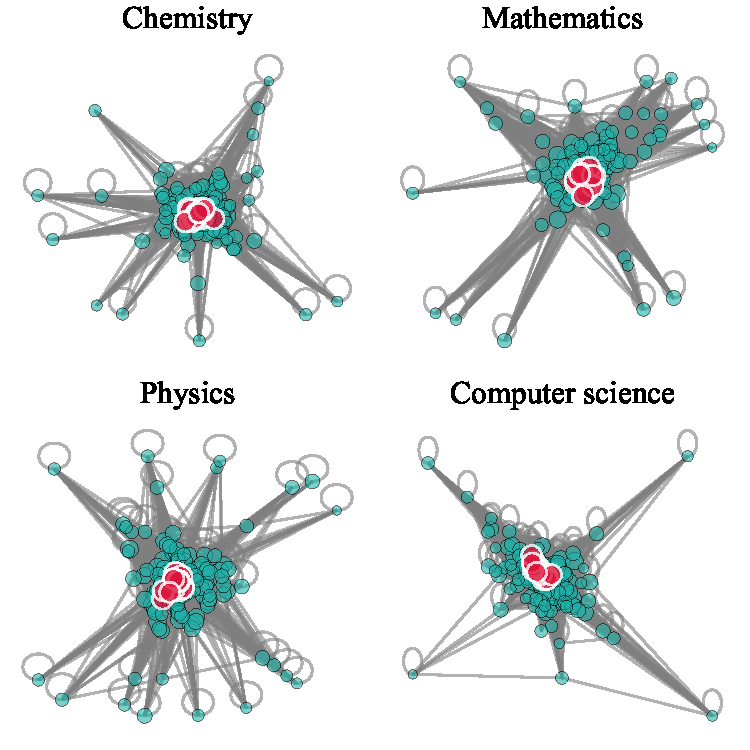
\includegraphics[width=0.45\textwidth]{figures/fig1.pdf}}
\caption{Network visualizations for chemistry, mathematics, physics and computer science fields showing central positions for institutions in the top 10 \% of prestige ranks (highlighted; higher institution has larger node size).}
\label{fig1}
\end{figure}


\subsection{Explore node features for the prediction task}
To better predict node property (prestige ranking of institutions), a series of node features are computed and explored for their relevance to the target. Selected node features are listed below:

(1) \textbf{Degree ratio}: The simplest measure of importance in a network is the number of connections in which some
vertex participates, i.e., the degree. The degree ratio $k_r$ is calculated by the out-degree $k_o$ (faculty production) and the in-degree $k_i$ (faculty consumption) according to $k_r = k_o / (k_o + k_i)$.

(2) \textbf{Degree centrality}: The degree centrality for a node $v$ is the fraction of nodes it is connected to. The degree centrality values are normalized by dividing by the maximum possible degree in a simple graph $n-1$ where $n$ is the number of nodes in the graph.

(3) \textbf{Eigenvector centrality}: Eigenvector centrality is a recursive measure of vertex “importance” in a network. A vertex with high eigenvector centrality is one to which other vertices with high
eigenvector centrality connect.

(4) \textbf{Harmonic centrality}: Important nodes in the network may be identified via geometric means, they are positioned more closely to all other vertices, with distances measured by geodesic (shortest) paths. Let $d_{uv}$ be the length of the shortest path from vertex $u$ to vertex $v$. The harmonic centrality is one of the related versions of geometric centrality, defined by
\begin{align}
h_c=\frac{1}{n-1} \sum_{u \neq v} \frac{1}{d_{u v}}
\end{align}

(5) \textbf{Closeness centrality}: It is another related version of geometric centrality, defined by
\begin{align}
c=\frac{1}{n} \sum_v d_{u v}
\end{align}

(6) \textbf{Betweenness centrality}: It is a measure of centrality in a graph based on shortest paths. The betweenness centrality for each vertex is the number of these shortest paths that pass through the vertex.

(7) \textbf{Clustering coefficients}: It is a measure of the degree to which nodes in a graph tend to cluster together. For directed graphs, the clustering is similarly defined as the fraction of all possible directed triangles or geometric average of the subgraph edge weights for unweighted and weighted directed graph respectively.

As shown in Fig.~\ref{fig2}, there is no direct correlation between individual node features and prestige rankings. For the degree centrality feature, its linear fit to prestige rankings has an $R^2$ value of about 0.65 on all 4 subsets. However, for the betweenness centrality feature, it only has an $R^2$ value of about 0.03 on all 4 subsets. There are some reasons can explain it: (1) node features may have complex relationships with node targets that are not captured by a simple linear relationship; (2) node features may contain irrelevant or noisy information that does not contribute much to predicting node targets; (3) the relationship between individual node features and node targets may not be apparent but becomes significant when considering their interactions; and (4) the dataset is not large enough and challenging to identify meaningful relationships between individual features and node targets.

\begin{figure}[htbp]
\centerline{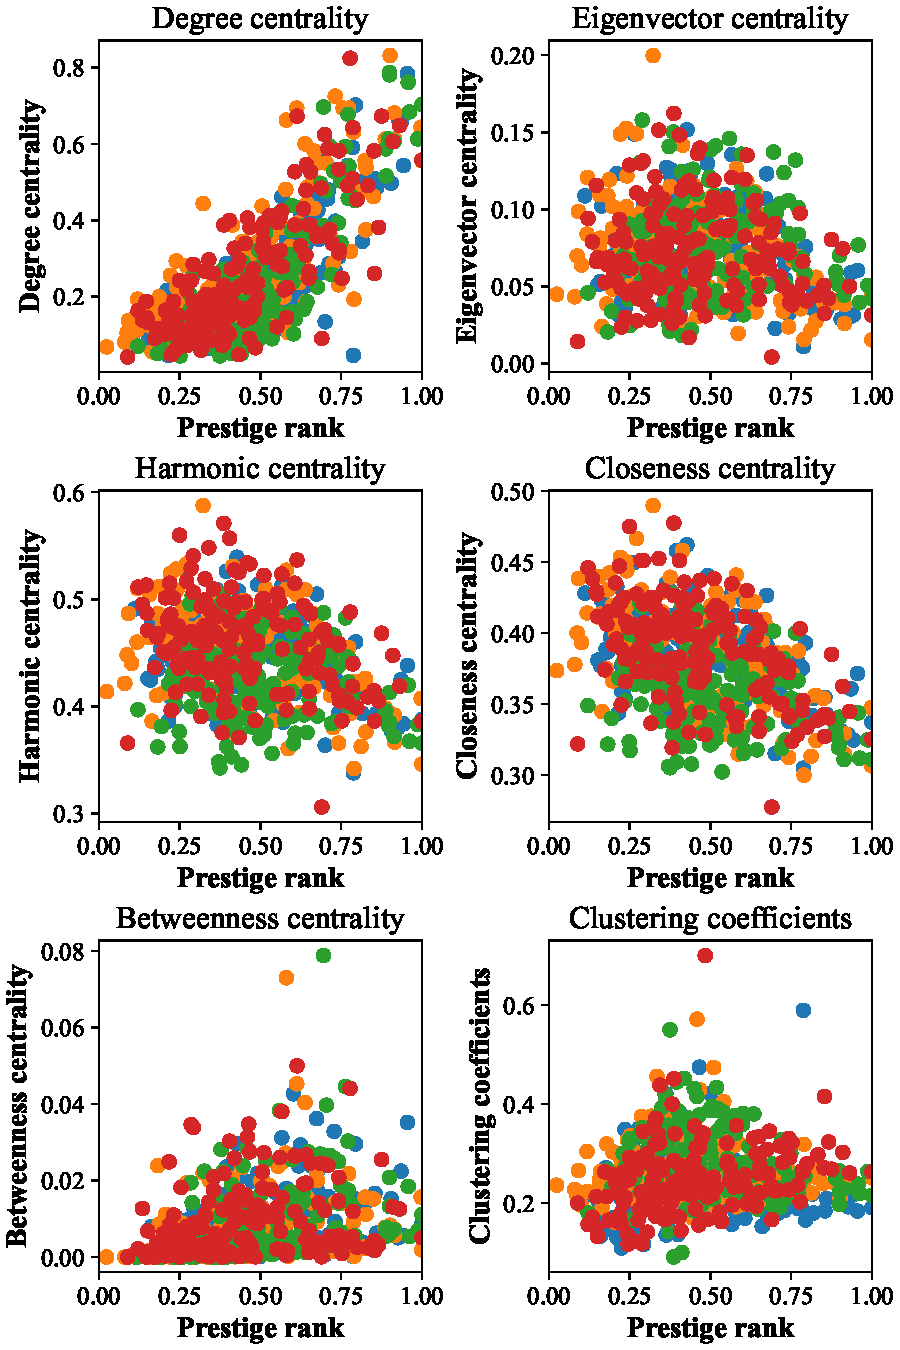
\includegraphics[width=0.48\textwidth]{figures/fig2.pdf}}
\caption{Distribution of various node features and prestige ranks, on the chemistry (blue), mathematics (orange), physics (green) and computer science (red) subsets}
\label{fig2}
\end{figure}


\section{Exploitation}


\subsection{GNN models}

\begin{table}[htbp]
\caption{The selected GNN models for ranking prediction.}
\begin{center}
\begin{tabular}{lc | lc }
\hline
\textbf{Model} & \textbf{Year} & \textbf{Model} & \textbf{Year}  \\
\hline
GCN  &  2016  &  UniMP  &  2020   \\
GraphSAGE  &  2017 & DeeperGCN  &  2020    \\
GAT  & 2017  & GATv2  &  2021     \\
GIN  & 2018  &   &     \\
\hline
\end{tabular}
\label{t2}
\end{center}
\end{table}

\begin{table*}[htbp]
\caption{Test $R^2$ scores of GNNs trained on the 4 subsets.}
\begin{center}
\begin{tabular}{lccccccc }
\hline
\textbf{Subset} & \textbf{GCN} & \textbf{SAGE} & \textbf{GIN} & \textbf{GAT} & \textbf{GATv2} & \textbf{UniMP} & \textbf{DeeperGCN}  \\
\hline
Chemistry  &  \textbf{0.95 (0.02)}  &  0.94 (0.02)  &  0.93 (0.02) & 0.93 (0.04) & 0.93 (0.02) & 0.93 (0.03) 
 & 0.92 (0.02) \\
Mathematics  &  \textbf{0.96 (0.01)} & 0.95 (0.01)  &  0.95 (0.02) & 0.94 (0.02) & 0.94 (0.02) & 0.95 (0.02)  
 & 0.95 (0.02) \\
Physics  & \textbf{0.94 (0.02)}  & 0.92 (0.03)  &  0.91 (0.04) & 0.90 (0.01) & 0.92 (0.03) & 0.90 (0.03) & 0.89 (0.03) \\
Computer science  & \textbf{0.92 (0.04)}  & 0.90 (0.05)  &  0.90 (0.04) & 0.85 (0.08) & 0.86 (0.05) & 0.85 (0.09) & 0.90 (0.04) \\
\hline
Average & \textbf{0.94} & 0.93 & 0.92 & 0.90 & 0.91 & 0.91 & 0.91 \\
\hline
\end{tabular}
\label{t3}
\end{center}
\end{table*}

Graph Neural Networks (GNNs) have achieved state-of-the-art performance on almost all tasks among various graph representation learning methods. According to the summary of the models used for node property prediction in OGB and other benchmarks, the representative GNN models between 2017-2022 are selected to predict the university rankings on the 4 subsets. The selected GNN models are listed in Table~\ref{t2}. Only the graph convolutional layers of these models are used to build the GNN models and predict the prestige rankings of  nodes on the 4 subsets. Thus, our architecture has 2 major components: graph convolutional layers and fully connected layers. Among them, the graph convolution layers of GCN and GIN are modified to use edge features in the message passing process. The edge features used in model training are edge weight and edge betweenness centrality.


\subsection{Experimental results}
In this work, all GNN models are trained and compared on all subsets under the same model hyperparameters and training conditions. The hyperparameters of the models are only briefly optimized rather than fully optimized, so the test results of the trained models are not necessarily the best performance that the models can achieve. All models were trained 10 times under different random seeds, and the results are shown in Table~\ref{t3}. The standard deviations of 10 experiments are in parentheses, and the best results of each subset are bolded. The results show that all models achieve $R^2$ scores around 0.9 or higher on the chemistry, mathematics and physics subsets. Half of the GNN models were unable to achieve $R^2$ scores higher than 0.9 on the computer science subset. Strangely, GCN achieves the best performance on all subsets, while state-of-the-art models such as UniMP and DeeperGCN perform poorly. This may be due to the large number of parameters of the new models, which is prone to overfitting on very small datasets. The results also show that the GCN model has the best performance and stability on all subsets.


\section{Conclusion}
Firstly, the USFHN dataset was divided according to different fields, and constructed chemistry, mathematics, physics and computer science subsets. On this basis, 7 kinds of node features were calculated, and it was found that there was no direct correlation between each individual node feature and prestige ranking. Among them, the degree centrality feature has a certain linear correlation with the ranking. Then, the graph convolutional layers of 7 reported GNNs were selected to build the model. These models are trained on all subsets under the same hyperparameters and training conditions. The results show that GCN has the best ranking prediction performance on all 4 subsets and surpasses new models such as GATv2.


\begin{thebibliography}{00}
\bibitem{b1} Clauset, A., Arbesman, S., Larremore, D. B. (2015). Systematic inequality and hierarchy in faculty hiring networks. Science advances, 1(1), e1400005.
\bibitem{b2} Wapman, K. H., Zhang, S., Clauset, A., Larremore, D. B. (2022). Quantifying hierarchy and dynamics in US faculty hiring and retention. Nature, 610(7930), 120--127.
\end{thebibliography}


\end{document}
